\documentclass[aspectratio=169, 11pt]{beamer}
\usetheme{Madrid}
\usecolortheme{beaver}

\usepackage[utf8]{inputenc}
\usepackage[T1]{fontenc}
\usepackage{amsmath,amssymb}
\usepackage{bm}
\usepackage{mathtools}
\usepackage{booktabs}
\usepackage{tabularx}
\usepackage{tikz}
\usepackage{hyperref}
\usepackage{multirow}
\usepackage[scale=0.9]{tgheros}

\usetikzlibrary{positioning, arrows, shapes, calc}
\tikzset{>=stealth}

\setbeamertemplate{navigation symbols}{}
\setbeamertemplate{footline}{}

\title[Media Recommender Systems]{Media Recommender Systems: \\ Spotify vs YouTube vs Netflix}
\subtitle{A Technical Deep Dive into Production-Grade Content AI}
\author{Intelligent Recommender Systems Course}
\date{\today}

\begin{document}

\begin{frame}
\titlepage
\end{frame}

\begin{frame}{Agenda}
\tableofcontents
\end{frame}

%=================================================================
\section{The Media Recommendation Problem}

\begin{frame}{Why Media Recommendation Is Fundamentally Different}
\begin{columns}[T]
\column{0.48\textwidth}
\small
\textbf{Job / E-commerce RS}
\begin{itemize}
    \item High-stakes, sparse interactions
    \item Long feedback cycles
    \item Multi-stakeholder optimization
\end{itemize}

\column{0.48\textwidth}
\small
\textbf{Media RS (Spotify, YouTube, Netflix)}
\begin{itemize}
    \item Low-stakes: wrong song $\to$ 30s skip
    \item Abundant implicit feedback (skips, dwell)
    \item Rapidly shifting tastes (minutes/hours)
\end{itemize}
\end{columns}

\vspace{0.2cm}
\centering
\small
\textbf{Key insight}: Media RS optimizes for \textbf{engagement and session depth}, with instant feedback on every recommendation.

\vspace{0.1cm}
\small
\textbf{Two-stage pipeline}: All three platforms use retrieval ($10^7\to10^2$) then ranking ($10^2\to10^1$).
\end{frame}

%=================================================================
\begin{frame}{Cold Start \& Content Understanding}
\small
\begin{columns}[T]
\column{0.48\textwidth}
\textbf{New User Solutions}:
\begin{itemize}
    \item Onboarding genre/artist picker
    \item Popularity + geo-based fallback
    \item Demographic collaborative filtering
\end{itemize}

\column{0.48\textwidth}
\textbf{New Item Solutions}:
\begin{itemize}
    \item Content-based features (audio/video/text)
    \item Metadata matching (genre, tags, cast)
    \item Explore-exploit via Thompson sampling
\end{itemize}
\end{columns}

\vspace{0.15cm}
\textbf{Feature extraction pipeline}:
\begin{equation*}
\mathbf{v}_{\text{item}} = \mathbf{W}_a\!\cdot\!\mathbf{v}_{\text{audio}} + \mathbf{W}_v\!\cdot\!\mathbf{v}_{\text{visual}} + \mathbf{W}_t\!\cdot\!\mathbf{v}_{\text{text}}
\end{equation*}

\begin{columns}[T]
\column{0.48\textwidth}
\small
\textbf{Spotify audio}: danceability, energy, valence, tempo, acousticness (from raw STFT $\to$ CNN)

\column{0.48\textwidth}
\small
\textbf{YouTube/Netflix video}: visual embeddings (ResNet), audio embeddings, scene detection, face recognition
\end{columns}
\end{frame}

%=================================================================
\section{Spotify's Architecture}

\begin{frame}{Spotify: Three Complementary Approaches}
\small
\textbf{Three pillars working together}:

\begin{center}
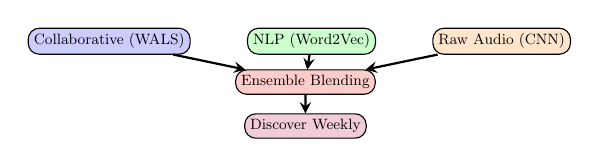
\begin{tikzpicture}[node distance=1cm, auto, every node/.style={font=\small}, scale=0.6, transform shape]
\node[draw, fill=blue!20, rectangle, rounded corners] (cf) {Collaborative (WALS)};
\node[draw, fill=green!20, rectangle, rounded corners, right=1.2cm of cf] (nlp) {NLP (Word2Vec)};
\node[draw, fill=orange!20, rectangle, rounded corners, right=1.2cm of nlp] (audio) {Raw Audio (CNN)};
\node[draw, fill=red!20, rectangle, rounded corners, below=0.6cm of $(cf)!0.5!(audio)$] (ensemble) {Ensemble Blending};
\node[draw, fill=purple!20, rectangle, rounded corners, below=0.4cm of ensemble] (final) {Discover Weekly};
\draw[->, thick] (cf)--(ensemble); \draw[->, thick] (nlp)--(ensemble);
\draw[->, thick] (audio)--(ensemble); \draw[->, thick] (ensemble)--(final);
\end{tikzpicture}
\end{center}

\vspace{0.1cm}
\textbf{Collaborative (WALS)}: $\displaystyle \min_{\mathbf{P},\mathbf{Q}} \sum c_{ui}(p_{ui} - \mathbf{p}_u\mathbf{q}_i)^2 + \lambda\|\mathbf{P},\mathbf{Q}\|^2$, with $c_{ui} = 1 + \alpha\cdot\text{play\_count}$

\vspace{0.1cm}
\textbf{NLP}: Word2Vec/Doc2Vec on blogs, forums, news $\to$ artist embedding space (cultural context)

\vspace{0.1cm}
\textbf{Raw Audio}: 3-layer CNN on STFT spectrogram $\to$ 128-dim embedding (genre, mood, instrumentation)

\vspace{0.1cm}
\textbf{Result}: 30 unique tracks/user/week in Discover Weekly, combining all three signals.
\end{frame}

%=================================================================
\begin{frame}{Spotify: Session-Based \& Skip Modeling}
\small
\textbf{Next-track prediction} (transition matrix):
\begin{equation*}
P(\text{track}_{t+1} \mid \text{track}_t) \propto \frac{\text{count}(t \to t+1)}{\text{count}(t \to \cdot)}
\end{equation*}

\vspace{0.1cm}
\textbf{GRU4Rec for session-based}:
\begin{equation*}
\mathbf{h}_t = \text{GRU}(\mathbf{h}_{t-1}, \mathbf{e}_{i_t}), \quad P(i_{t+1}) = \text{softmax}(\mathbf{W} \cdot \mathbf{h}_t)
\end{equation*}

\vspace{0.1cm}
\textbf{Skip signal modeling}:
\begin{itemize}
    \item Early skip ($<10s$): wrong recommendation entirely
    \item Late skip ($>60\%$): lost interest, context mismatch
    \item Context-aware: morning commute (+15\% skip), gym (-20\%)
\end{itemize}

\vspace{0.1cm}
\textbf{Multi-task learning}:
\begin{equation*}
\mathcal{L} = \mathcal{L}_{\text{play}} + \lambda_{\text{skip}} \mathcal{L}_{\text{skip}} + \lambda_{\text{dwell}} \mathcal{L}_{\text{dwell}}
\end{equation*}

\textbf{Skip-aware ranking}:
\begin{equation*}
\text{RankScore} = \text{Score}_{\text{base}} - \beta \cdot P(\text{skip} \mid u,i,\text{ctx})
\end{equation*}
\end{frame}

%=================================================================
\section{YouTube's Architecture}

\begin{frame}{YouTube: Two-Tower DNN for Candidate Generation}
\small
\textbf{Two-tower neural retrieval}:

\begin{align*}
\mathbf{e}_u &= f_\theta(\text{watch\_hist}, \text{search}, \text{demographics}) \in \mathbb{R}^d \\
\mathbf{e}_v &= g_\phi(\text{video\_feats}, \text{channel}, \text{tags}) \in \mathbb{R}^d
\end{align*}

\textbf{Score}: $\displaystyle \text{score}(u,v) = \cos(\mathbf{e}_u, \mathbf{e}_v)$

\vspace{0.1cm}
\textbf{Training}: Sampled softmax with millions of negatives:
\begin{equation*}
\mathcal{L} = -\sum_{(u,v^+)} \log \frac{e^{\cos(\mathbf{e}_u,\mathbf{e}_{v^+})}}{\sum_{v \in \mathcal{N}(u)} e^{\cos(\mathbf{e}_u,\mathbf{e}_v)}}
\end{equation*}

\vspace{0.1cm}
\textbf{Key design choices}:
\begin{itemize}
    \item Watch history: average of last 50 video embeddings
    \item Example age: feature decay for freshness bias
    \item Hashing trick for sparse ID compression
\end{itemize}

\vspace{0.1cm}
\textbf{Candidate sources}: DNN retrieval + popularity + geo + channel subscriptions $\to$ hundreds of candidates.
\end{frame}

%=================================================================
\begin{frame}{YouTube: Wide \& Deep Ranking with Watch-Time Optimization}
\small
\textbf{Wide \& Deep} (Google, 2016):
\begin{equation*}
\hat{y} = \sigma(\underbrace{\mathbf{w}_{\text{wide}}^T \mathbf{x}_{\text{wide}}}_{\text{memorization}} + \underbrace{\text{MLP}(\mathbf{x}_{\text{deep}})}_{\text{generalization}})
\end{equation*}

\vspace{0.1cm}
\textbf{Wide}: cross-product transformations (e.g., "user watched X AND video from channel Y")

\textbf{Deep}: 3 hidden layers (1024$\to$512$\to$256) with ReLU

\vspace{0.1cm}
\textbf{Watch-time optimization} (not CTR!):
\begin{itemize}
    \item Label: $\text{watch\_time} / \text{video\_duration}$
    \item Weighted logistic: $w_i = \text{observed watch time}$
    \item Model estimates $\mathbb{E}[\text{watch\_time}]$
\end{itemize}

\vspace{0.1cm}
\begin{equation*}
\mathcal{L} = -\sum_i w_i\bigl[y_i\log\hat{y}_i + (1-y_i)\log(1-\hat{y}_i)\bigr]
\end{equation*}

\vspace{0.1cm}
\textbf{Result}: +81\% watch time uplift (Covington et al., 2016). Clickbait dies because short watch = low weight.
\end{frame}

%=================================================================
\section{Netflix's Architecture}

\begin{frame}{Netflix: Contextual Ranking \& Personalization}
\small
\textbf{Three-tier personalization}:
\begin{enumerate}
    \item \textbf{Which titles}: two-tower retrieval (user $\times$ context)
    \item \textbf{How to show}: artwork personalization per user
    \item \textbf{Row ordering}: which genre rows appear
\end{enumerate}

\vspace{0.15cm}
\textbf{Contextual ranking}:
\begin{equation*}
P(\text{play} \mid u, i, \text{ctx}) = \sigma(\mathbf{w}^T \cdot [\phi_{\text{personal}}(u,i) \oplus \phi_{\text{ctx}}(t) \oplus \phi_{\text{popular}}(i)])
\end{equation*}

\vspace{0.1cm}
\textbf{Context signals}: time of day (morning: short), day of week (weekend: binge), device (mobile $\neq$ TV), group vs solo

\vspace{0.15cm}
\textbf{Artwork personalization}:
\begin{itemize}
    \item Same movie, different poster per user
    \item Action fan $\to$ explosions; romance fan $\to$ couple
    \item Scene detection $\to$ emotion classifier $\to$ user preference match
    \item Result: +0.3\% engagement at scale
\end{itemize}
\end{frame}

%=================================================================
\section{The Skip \& Engagement Problem}

\begin{frame}{Why Users Skip — Modeling Negative Feedback}
\small
\textbf{Skip rates by platform}: Spotify $\sim$30\% within 10s, YouTube $\sim$40\% within 30s, Netflix $\sim$20\% within 5min.

\begin{columns}[T]
\column{0.48\textwidth}
\textbf{Skip classification}:
\begin{align*}
\text{Satisfied: } &\text{dwell} > 70\% \\
\text{Partial: } &\text{dwell} \in [30\%, 70\%] \\
\text{Rejected: } &\text{dwell} < 30\%
\end{align*}

\vspace{0.1cm}
\textbf{Censored dwell model}:
\begin{equation*}
P(\text{dwell} > t) = \exp\!\left(-\frac{t}{\mu(u,i)}\right)
\end{equation*}

\column{0.48\textwidth}
\textbf{Skip timing patterns}:
\begin{itemize}
    \item Early skip ($<10s$): $\to$ wrong recommendation
    \item Mid skip ($10s-60s$): $\to$ okay but not engaging
    \item Late skip ($>60\%$): $\to$ context changed
\end{itemize}

\vspace{0.1cm}
\textbf{Context matters}: same user, same song, different time = different skip probability.
\end{columns}

\vspace{0.15cm}
\textbf{Dwell-weighted training}:
\begin{equation*}
\text{weight}_{ui} = \frac{\min(\text{dwell}_{ui}, \text{cap})}{\text{duration}_i} \in [0, 1]
\end{equation*}
A 30s dwell on a 3min song = 0.17 weight. A full play = 1.0.
\end{frame}

%=================================================================
\section{Algorithmic Approaches}

\begin{frame}{Content-Based \& CF for Media}
\small
\begin{columns}[T]
\column{0.48\textwidth}
\textbf{Content-Based}:
\begin{align*}
\mathbf{p}_u &= \frac{1}{|I_u^+|}\sum \mathbf{v}_i^{\text{tfidf}} \\
\text{sim}_{\text{audio}}(i,j) &= \cos(\mathbf{a}_i, \mathbf{a}_j)
\end{align*}
Multi-modal fusion beats single modality:
\begin{table}
\centering
\small
\begin{tabular}{lc}
\toprule
\textbf{Method} & \textbf{Recall@10} \\
\midrule
TF-IDF only & 0.38 \\
Audio CNN & 0.55 \\
Multi-modal fusion & \textbf{0.68} \\
\bottomrule
\end{tabular}
\end{table}

\column{0.48\textwidth}
\textbf{Collaborative Filtering}:
\begin{align*}
\hat{r}_{u,i} &= \mu + b_u + b_i + \mathbf{p}_u\mathbf{q}_i \\
s_{i,j}^{\text{item}} &= \frac{|U_i \cap U_j|}{|U_i \cup U_j|}
\end{align*}

\textbf{Sequential (BERT4Rec)}:
\begin{equation*}
P(i_t \mid i_{<t}, i_{>t}) = \text{softmax}(\mathbf{W} \cdot \text{BERT}(\mathbf{E})_t)
\end{equation*}

\textbf{Hybrid score}:
\begin{equation*}
\text{Final} = \alpha\,\text{CB} + \beta\,\text{CF} + \gamma\,\text{KB}
\end{equation*}
\end{columns}
\end{frame}

%=================================================================
\section{Evaluation \& Fairness}

\begin{frame}{Evaluation \& The Filter Bubble}
\small
\begin{columns}[T]
\column{0.48\textwidth}
\textbf{Offline metrics}:
\begin{align*}
\text{Recall@k} &= \frac{|\text{rel} \cap \text{top-k}|}{|\text{rel}|} \\
\text{Skip Rate} &= \frac{\#\text{skips}}{\#\text{plays}} \\
\text{Session Depth} &= \text{avg items/session} \\
\text{Coverage} &= \frac{|\text{rec items}|}{|\text{total items}|}
\end{align*}

\textbf{A/B metrics by platform}:
\begin{itemize}
    \item Spotify: session time, skip rate
    \item YouTube: watch time, session depth
    \item Netflix: 30-day retention
\end{itemize}

\column{0.48\textwidth}
\textbf{Filter bubble problem}:
\begin{itemize}
    \item Popularity bias: rich get richer
    \item Position bias: top = more clicks
    \item Echo chambers: never discover new genres
\end{itemize}

\textbf{Solutions}:
\begin{align*}
\text{Score}' &= \text{Score} - \gamma \cdot \log(\text{pop}_i) \\
\text{MMR} &= \max_i [ \text{rel}(i) - \lambda \cdot \max_{j\in S} \text{sim}(i,j) ]
\end{align*}

\textbf{Fairness constraints}:
\begin{equation*}
P(\text{rec} \mid \text{genre}_A) = P(\text{rec} \mid \text{genre}_B)
\end{equation*}
\end{columns}
\end{frame}

%=================================================================
\section{The Future}

\begin{frame}{Generative AI \& Summary}
\small
\begin{columns}[T]
\column{0.48\textwidth}
\textbf{Next frontier}:
\begin{itemize}
    \item Matching $\to$ Creating: AI-generated personalized tracks
    \item AI DJ (Spotify): LLM commentary between songs
    \item Facial expression $\to$ mood $\to$ music matching
\end{itemize}

\vspace{0.15cm}
\textbf{Architecture}: RAG for media
\begin{equation*}
\text{Playlist} = \text{LLM}(\text{query} \oplus \text{retrieved} \oplus \text{taste})
\end{equation*}

\column{0.48\textwidth}
\textbf{Platform comparison}:
\begin{table}
\centering
\small
\begin{tabular}{lll}
\toprule
\textbf{Dimension} & \textbf{Spotify} & \textbf{YouTube} \\
\midrule
Signal & Audio + NLP + CF & Watch history \\
Ranking & Ensemble blending & Wide \& Deep \\
Goal & Engagement + discovery & Watch time \\
Skip & Contextual model & Dwell regression \\
\midrule
& \textbf{Netflix} & \\
& Context + artwork & \\
& Contextual DNN & \\
& Retention & \\
& Abandonment model & \\
\bottomrule
\end{tabular}
\end{table}
\end{columns}

\vspace{0.1cm}
\centering
\textbf{Bottom line}: Same retrieve$\to$rank paradigm, different signals and optimization targets.
\end{frame}

%=================================================================
\begin{frame}
\centering
\Huge Questions \& Discussion

\vspace{0.5cm}
\normalsize
Thank you for your attention.
\end{frame}

\end{document}
